\documentclass[11pt]{article}
\usepackage{icmlko}
\begin{document}

\title{막았더니 더 나빠졌다 --- 표지가 하나여야 하는 이유를 세 번째로 못 찾았다}
\author{월드모델 실험실}
\date{노트 422 · 2026년 8월 2일}
\maketitle

\begin{abstract}
노트 421이 노트 420의 설명을 물리면서 새 설명을 냈다 --- \emph{표지 둘이
해로운 건 칸 수가 아니라 나무가 둘을 \textbf{곱해서} 도메인을 콕 집기
때문이다.} 그 설명은 곧바로 처방을 준다: \textbf{곱만 막으면} 둘 다 얻는다.

막았다. F18 은 자루를 서른둘 친다 --- \textbf{절반은 grp 만, 절반은 grp2 만}
보게 하고(못 보는 쪽은 중립 $0.5$ · 표시자 $0$ 으로 가림) 예측 때도 같은
가림을 썼다. 어느 나무도 둘을 같이 못 보므로 곱이 안 생긴다.

\begin{center}
\begin{tabular}{lr}
\hline
 & KR 만화 전이 \\
\hline
\textbf{표지 하나} (챔피언) & $\mathbf{+0.1946}$ \\
표지 둘, 곱 허용 & $+0.0819$ \\
\textbf{표지 둘, 곱 막음} & $\mathbf{+0.0064}$ \\
\hline
\end{tabular}
\end{center}

\textbf{막았더니 더 나빠졌다.} 곱을 허용한 쪽($+0.0819$)보다도 낮다.
사전 등록에 적어 둔 실패 조건이 그대로다 --- \emph{전이가 그래도 내려가면
곱이 아니다; grp2 의 정보 자체가 안 본 도메인에 해로운 것이고 노트 421의
설명도 물러야 한다.}
\end{abstract}

\section{세 번째로 못 찾았다}

같은 물음(\emph{왜 표지는 하나여야 하나})에 설명이 셋 죽었다.

\begin{center}
\begin{tabular}{lll}
\hline
설명 & 낸 곳 & 어떻게 죽었나 \\
\hline
칸을 더 늘려서 & 노트 420 & 잘게 하면 오히려 이롭다(노트 421) \\
나무가 둘을 곱해서 & 노트 421 & 막았더니 더 나쁘다(여기) \\
\hline
\end{tabular}
\end{center}

노트 385가 달력에 대해, 노트 414가 웹툰에 대해 한 처분을 여기에도 쓴다 ---
\textbf{관측으로 둔다.}

\begin{center}
\textbf{도메인 표지는 하나만 쓴다. 왜인지는 모른다.}
\end{center}

값은 이미 재어 놓았다(노트 420): 둘째를 넣으면 판 $+0.0035$ 를 얻고 전이
$-0.1140\ [-0.159, -0.067]$ 을 낸다. 규약이 그것을 막는다.

\section{이 측정의 한계}

\texttt{SplitBag} 은 곱만 막은 것이 아니다 --- \textbf{표지마다 자루가
열여섯 개}로 준다(원래는 서른둘이 다 본다). 그래서 분산이 는다. 전이가
내린 데에 그 몫이 섞여 있다.

다만 \textbf{분산만으로는 이 값이 안 나온다.} 분산이 원인이라면 결과가 두
팔 \emph{사이}에 놓여야 하는데, $+0.0064$ 는 \textbf{둘 다보다 낮다}.
반씩 본 두 무리가 서로 다른 줄을 세우고, 그 둘을 순위로 평균하면 어느 쪽도
아닌 것이 나오는 쪽에 가깝다.

\section{남은 것}

\begin{tabular}{lp{7.0cm}}
\hline
표지의 ``질'' & 갈래 수도(421) 곱도(422) 아니었다. 남은 뜻은
\textbf{어느 field 를 쓰느냐} 하나다 --- grp 의 여덟 자리를 바꿔 가며
재는 것 \\
반씩 본 두 무리의 불일치 & 위 한계를 뒤집으면 측정이 된다 --- 두 무리가
같은 유보 행을 얼마나 다르게 세우나 \\
챔피언 & 안 바뀐다 \\
\hline
\end{tabular}

\begin{figure}[h]
\centering
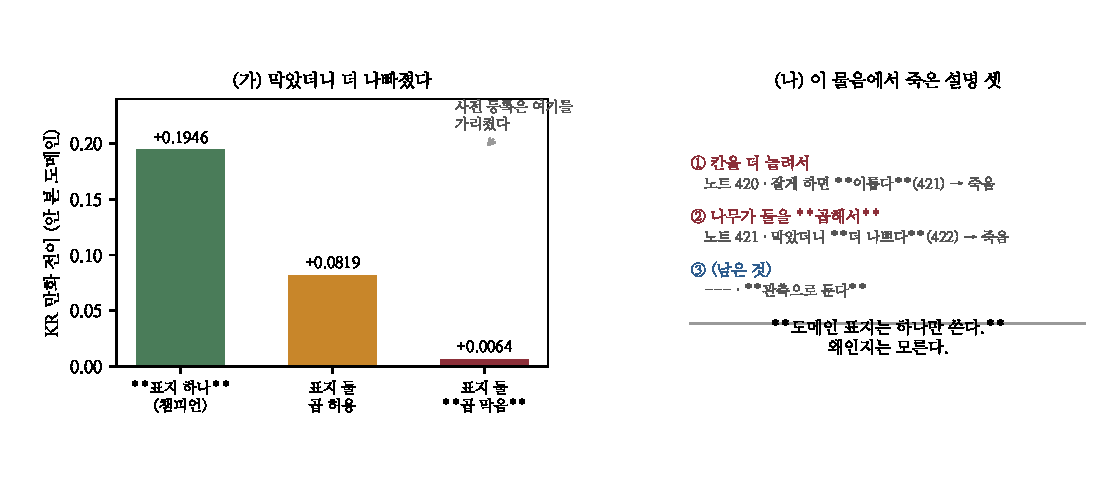
\includegraphics[width=\textwidth]{figs/fig422.pdf}
\caption{(가) 곱을 막으면 전이가 더 내린다 --- 사전 등록은 챔피언 높이를
가리켰다. (나) 같은 물음에서 죽은 설명 셋.}
\end{figure}

\end{document}
